\section{Sprung}
In diesem Teil wird die Sprungantwort der 3 Tiefpässe untersucht. Der Filter wird mit einem Rechtecksignal der Amplitude $\SI{6}{\volt}$ und Frequenz $\SI{2000}{\hertz}$  angeregt und ein Oszilloskop erfasst das Ausgangssignal.

%%%%%%%%%%%%%%%%%%%%%%%%%%%%%%%%%%%%%%%%%%%%%%%%Comments
%Plots der Sprungantworten der drei Tiefpässe, Bestimmung von Anstiegszeit, Überschwingen und Einschwingzeit; Darstellung und Vergleich in einer Tabelle
%multi figure

\begin{figure}[H]
\begin{center}
\subfloat[Bessel]{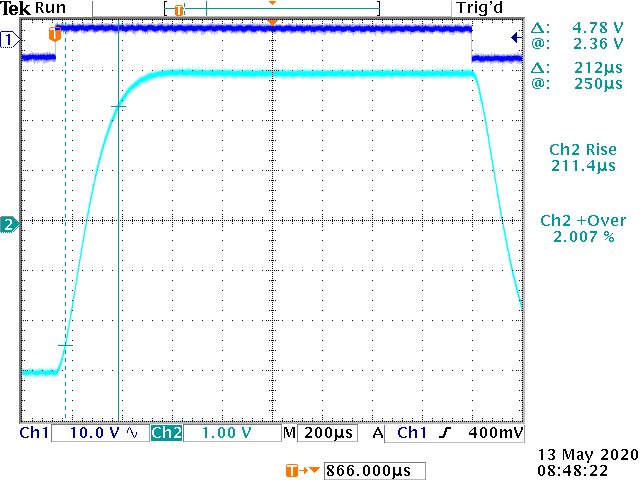
\includegraphics[width = \textwidth/3]{img/4 Bessel Anstiegszeit.png}}  
\subfloat[Butterworth]{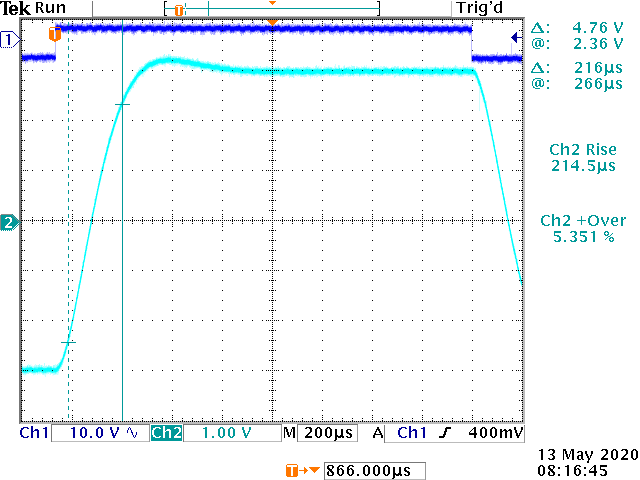
\includegraphics[width = \textwidth/3]{img/4 Butterworth Anstiegszeit .png}} 
\subfloat[Tschebyscheff]{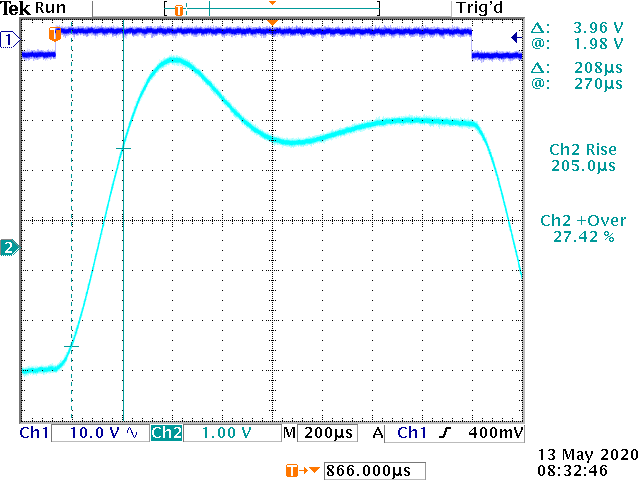
\includegraphics[width = \textwidth/3]{img/4 Tscheby Anstiegszeit.png}} \\
%\subfloat[\imgfilename]{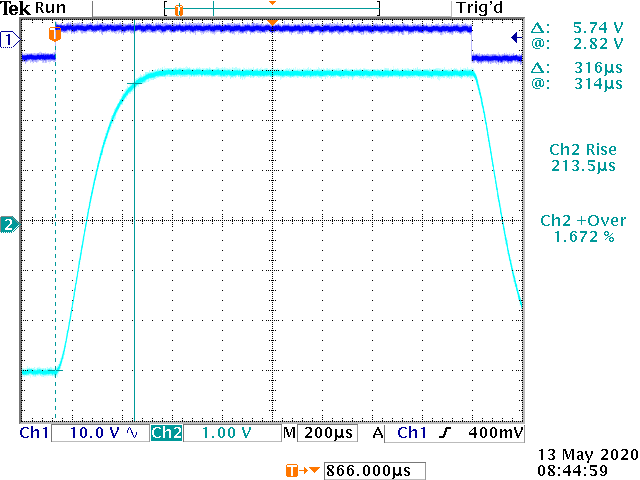
\includegraphics[width = \textwidth/3]{img/4 Bessel Einschwingzeit.png}}  
%\subfloat[\imgfilename]{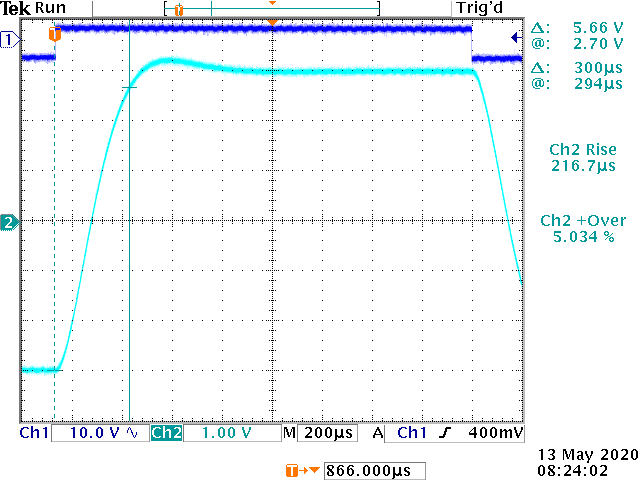
\includegraphics[width = \textwidth/3]{img/4 Butterworth Einschwingzeit.png}} 
%\subfloat[\imgfilename]{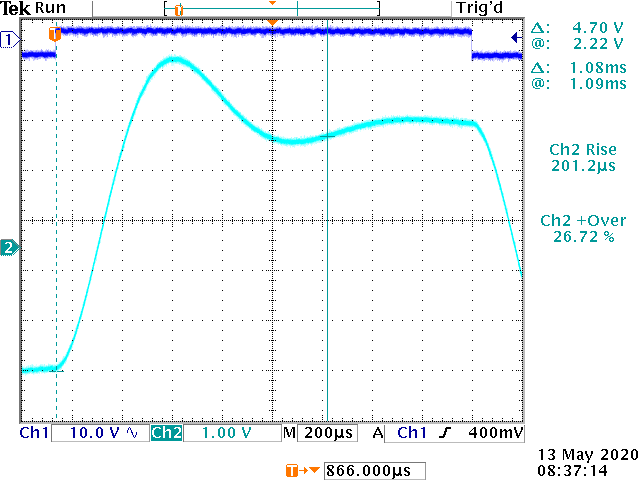
\includegraphics[width = \textwidth/3]{img/4 Tscheby Einschwingzeit.png}} \\
%\subfloat[\imgfilename]{\includegraphics[width = \textwidth/3]{img/4 Bessel Überschwingzeit.png}}  
%\subfloat[\imgfilename]{\includegraphics[width = \textwidth/3]{img/4 Butterworth Überschwingen.png}} 
%\subfloat[\imgfilename]{\includegraphics[width = \textwidth/3]{img/4 Tscheby Überschwingzeit.png}} \\
%\caption{Anstiegszeit, Einschwingzeit und Überschwingzeit}
\label{fig:A4_mult}
\end{center}
\end{figure}

In der \autoref{fig:A4_mult} sind die Anstiegszeit, Einschwingzeit und das Überschwingen abgebildet. Die Werte aus der Folgenden Tabelle stammen aus der Anlage: "GNP V3 Messwerte (Tabelle).pdf".

\begin{table}[H]
    \centering
    \begin{tabular}{|c|c|c|c|c|}\hline
    \tbf{Filter} & \tbf{Anstiegszeit} & \tbf{Überschwingen}     &  \tbf{Einschwingen}     & \tbf{Ausgangsamplitude}   \\ \hline
    Butterworth                   & \SI{216}{\micro\second} &     \SI{0.26}{\volt} &\SI{300}{\micro\second} & \SI{6}{\volt_{pp}}   \\
    Tschebyscheff             & \SI{208}{\micro\second}  &    \SI{1.2}{\volt}  &\SI{1.08}{\milli\second} & \SI{5}{\volt_{pp}}   \\ 
    Bessel                &\SI{212}{\micro\second}  & \SI{40}{\milli\volt} &\SI{316}{\micro\second} &\SI{6}{\volt_{pp}} \\ \hline
    \end{tabular}
    \caption{Grenzfrequenzen der Filter}
\end{table}

\subsection{Auswertung}
Die Filter verhalten sich wie erwartet. Der Bessel Filter gibt das Rechtecksignal am genausten wieder, Butterworth und Tschebyscheff überschwingen, der Tschebyscheff mit einem zweiten negativen Überschwinger. Die Einschwingzeit von dem Teschbyscheff Filter liegt mit $\SI{1.08}{\milli\second} $ weitaus höher als Butterworth und Bessel mit $\SI{300}{\micro\second}$ und $\SI{316}{\micro\second}$. %intressant zu erwähnen warum Teschbyscheff 5vpp und nicht 6vpp hat?
Butterworth und Bessel unterscheiden sich in ihrer antwort, auf das Rechtecksignal, relativ wenig. Das überschwingen ist der entscheidende faktor den die beiden Filter von einander Trennt. Mit $\SI{0.26}{\volt}$ ist die höhe des Überschwingens vier mal so hoch beim Butterworth im Vergleich zum Bessel Filter.